\section{第3讲\quad 行程问题与应用题}

\item {
    【追及】
    猎豹跑一步长为2米,狐狸跑一步长为1米. 猎豹跑2步的时间狐狸跑3步. 猎豹距离狐狸30米,则猎豹跑动\underline{\hbox to 20mm{}}米可追上狐狸. 
    \ifshowSolution 
        \fangsong\zihao{5}\textcolor{blue}{
            \\正解: 120m.\\
                不妨假设猎豹1秒跑2步,那么狐狸1秒跑3步;\\
                那么,猎豹的速度是 \[2\times 2 = 4m/s,\] 
                狐狸的速度是 
                \[1\times 3 = 3 m/s.\]
                \[距离\div 速度差 = 追及所需时间\]
                \[30\div (4-3) = 30(s). \]
                \[30 \times 4 = 120 (m).\]
        }
    \else
        \vspace{2cm}
    \fi
    % 2017年第二十二届“华罗庚金杯”少年数学邀请赛初赛试卷(小中组).doc, 120
}

\item {
    【相遇】
    一辆公共汽车和一辆小轿车同时从相距450千米的两地相向而行,公共汽车每小时行40千米,小轿车每小时行50千米,\underline{\hbox to 20mm{}}小时后两车第二次相距90千米. 
    \ifshowSolution 
        \fangsong\zihao{5}\textcolor{blue}{
            \\正解: \\
                第2次相遇时,两车一共走 \[450+90=540 km;\]
                \[540\div (40+50) = 6h.\]
        }
    \else
        \vspace{2cm}
    \fi
    % 2020数学花园探秘笔试小中决赛D卷.doc; 6
}

\item {
    【相遇】
    里山镇到省城的高速路全长189千米,途径县城. 县城离里山镇54千米. 早上8: 30一辆客车从里山镇开往县城,9: 15到达. 停留15分钟后开往省城,午前11: 00能够到达. 另有一辆客车于当日早上9: 00从省城径直开往里山镇. 每小时行驶60千米. 两车相遇时,省城开往里山镇的客车行驶了\underline{\hbox to 20mm{}}分钟.
    \ifshowSolution 
        \fangsong\zihao{5}\textcolor{blue}{
            \\正解: \\
            \begin{figure}[H] 
                \centering
                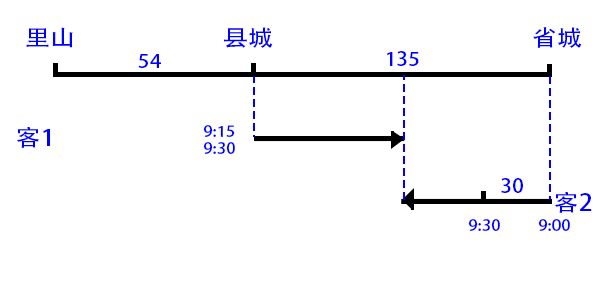
\includegraphics[width=0.6\textwidth]{./pics/Chapter_3/seikai_1.png}
            \end{figure}
                从里山开往省城的客车,9:30从县城出发,县城到省城段速度:
                    \[11:00 - 9:30 = 1.5 h\]
                    \[(189-54)\div 1.5=90 km/h\]
                9:00到9:30, 从省城出发的客车行驶了0.5h,行驶距离:
                    \[60\times 0.5 = 30km\]
                所以,在9:30两车相距
                    \[135 - 30 = 105 km\]
                两车相遇还需要
                \[105\div (90+60) = 0.7h,\]
                此时,从省城出发的客车行驶了
                \[0.5 + 0.7 = 1.2(h) = 72(min).\]
        }
    \else
        \vspace{2cm}
    \fi
    % 2012年第十七届“华罗庚金杯”少年数学邀请赛网上初赛试卷(小学中低年级组).doc, 72
}

\item {
    【多次追及】
    哥哥和弟弟两人同时从家出发去 2000米外的学校上学,哥哥每分钟走 60米,弟弟每分钟走 50 米,走了 10 分钟后,哥哥发现忘记带数学错题本,就以每分钟 100 米的速度跑回家,回到家后,哥哥用了2分钟找到了错题本,然后以每分钟 150 米的速度往学校跑.从哥哥第二次从家出发开始计算,经过\underline{\hbox to 20mm{}}分钟后,哥哥能追上弟弟.
    \ifshowSolution 
        \fangsong\zihao{5}\textcolor{blue}{
            \\正解: \\
            \begin{figure}[H] 
                \centering
                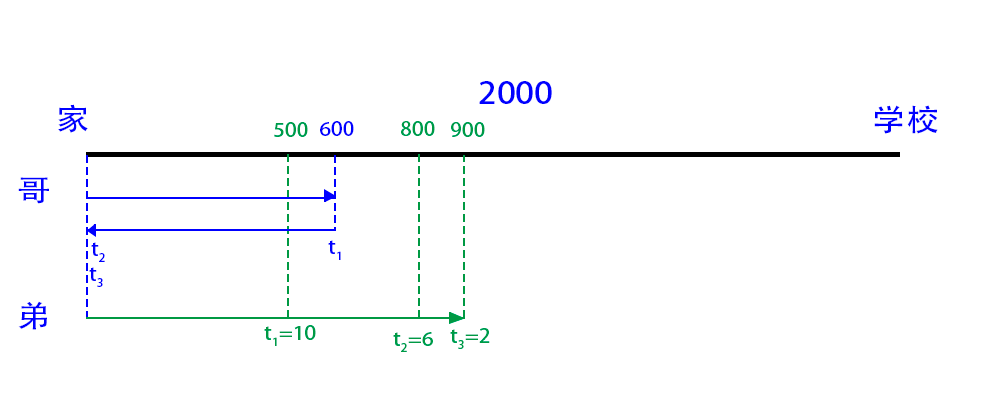
\includegraphics[width=0.7\textwidth]{./pics/Chapter_3/seikai_2.png}
            \end{figure}
                从哥哥第一次从家里出发,到再次出发,经过的时间如下.\\
                $t_1=10 min$: 第一次出发到发现忘带本子;此时哥哥走了
                \[60\times 10 = 600 (m).\]
                $t_2=600\div 100 = 6(min)$: 从发现忘带本子到跑回家.\\
                $t_3=2(min)$: 到家找到本子第二次从家里出发.\\
                在以上时间内,弟弟都以50m/min 的速度向学校走去,共走了
                \[ 50\times (10+6+2) = 900 m.\]
                哥哥第二次从家里出发,需要
                \[900\div (150 - 50) = 9 min \]
                追上弟弟.
        }
    \else
        \vspace{2cm}
    \fi
    % 2020华数之星初赛-三四年级真题.pdf; 9
}

\item {
    【多次相遇】
    甲、乙两人在一条长120米的直路上来回跑,甲的速度是5米/秒,乙的速度是3米/秒,若他们同时从同一端出发跑了15分钟,则他们在这段时间内共迎面相遇\underline{\hbox to 20mm{}}次(端点除外). 
    \ifshowSolution 
        \fangsong\zihao{5}\textcolor{blue}{
            \\正解: \\
                甲乙两人迎面相遇时,2人一共的行程是2个单程:
                $$120\times 2=240(米)$$
                用时为
                $$240\div (3+5)=30(秒)$$
                即每30秒就相遇一次(包括端点相遇).
                端点相遇用时为:
                甲单程用时:
                 $$120\div 3 = 40 (s),$$
                乙单程用时:
                $$120\div 5=24 (s)$$
                两人迎面相遇的时间为40和24的公倍数,最小公倍数是120.
                $$120\div 30=4$$
                可知,他们4次相遇中就有1次为端点相遇,
                即15分钟内相遇的总次数为:
                 $$15\times 60\div 30 = 30(次),$$
                其中在端点相遇的次数为 $30\div 4$ 的整数部分即7.
                所以他们在这段时间内共迎面相遇(端点除外)的次数为:
                $$30-7=23(次).$$
        }
    \else
        \vspace{2cm}
    \fi
    % 2015华, 23
}

\item {
    【多次相遇】
    甲、乙两车分别从A,B两地同时出发,相向匀速行进,在距A地 60 千米处相遇. 相遇后,两车继续行进,分别到达B,A后, 立即原路返回, 在距B地50 千米处再次相遇. 则A,B两地的路程是\underline{\hbox to 20mm{}}千米. 
    \ifshowSolution 
        \fangsong\zihao{5}\textcolor{blue}{
            \\正解:
            \begin{figure}[H] 
                \centering
                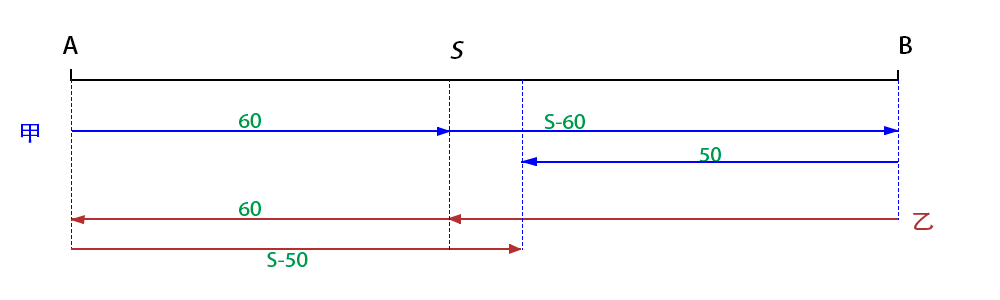
\includegraphics[width=0.7\textwidth]{./pics/Chapter_3/seikai_3.png}
            \end{figure}
            相遇时距离之比等于速度之比.\\
            设AB两地间的距离为S km.\\
            第一次相遇时,甲走了 60千米,而乙走了S-60 千米; \\
            第二次相遇,甲又走了S-60+50千米,乙又走了60+S-50千米.\\
            \begin{align*}
                \frac{60}{S-60} &= \frac{S-60+50}{60+S-50} \\
                S&=130.
            \end{align*}
        }
    \else
        \vspace{2cm}
    \fi
    % 2016华, 130
}

\item {
    【多次相遇】
    甲、乙两车分别从A,B两地同时出发,相向而行,3小时后相遇,甲掉头返回A地,乙继续前行. 甲到达A地后掉头往B行驶,半小时后和乙相遇. 那么乙从A到B共需\underline{\hbox to 20mm{}}小时.
    \ifshowSolution 
        \fangsong\zihao{5}\textcolor{blue}{
            \\正解:\\ 
                相遇后,甲还需要3小时返回甲地,\\
                第二次相遇时,甲距离第一次相遇点的距离等于甲 2.5 小时的路程,乙用了3.5小时走这些路程,所以甲乙速度的比是7:5,\\
                甲乙相遇需要3小时,那么乙单独到需要
                \[ 3\times \frac{7+5}{5} = 7.2小时.\]
        }
    \else
        \vspace{2cm}
    \fi
    % 2011年第十六届“华罗庚金杯”少年数学邀请赛初赛试卷(小学组).doc, 7.2
}

\item {
    【行程与时间计算】
    小文今天和朋友约定一起看 12:00 开场的电影,出门时,发现挂钟电池没电已经停止了,她把挂钟换好电池,但没来得及调整时间,出门前挂钟显示的时间是 9:25,小文赶到电影院时,电影刚好开场.电影结束后,小文立刻返回家中,发现挂钟显示的时间是 13:55,小文赶紧把它调成正确的时间15:45.如果小文从家到电影院和从电影院返回家中花的时间是一样的,那么,电影的时长是\underline{\hbox to 20mm{}}分钟.
    \ifshowSolution{}
        \fangsong\zihao{5}\textcolor{blue}{
            \\正解:
            \begin{figure}[H] 
                \centering
                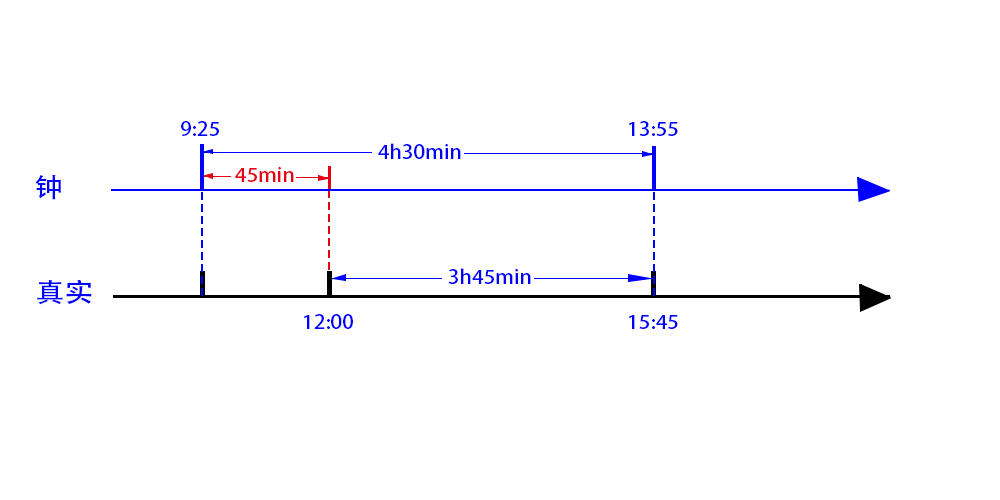
\includegraphics[width=0.7\textwidth]{./pics/Chapter_3/seikai_8.png}
            \end{figure}
            钟从 9:25到13:55(真实时间为15:45),用时 
            \[ 13:55 - 9:25 = 4h 30 min. \]
            真实时间从12:00 到 15:45, 用时
            \[ 15:45 - 12:00 = 3h 45 min. \]
            钟9:25到真实12:00, 用时
            \[
                4h 30min - 3h 45 min = 45min
            \]
            所以,电影时长:
            \[3h 45min - 45min = 3h = 180min. \]
        }
    \else
        \vspace{2cm}
    \fi
    % 迎春杯四年级2022-试卷.pdf; 180
}

\item {
    【流水行船·追及·相遇】
    一条河上有A,B两个码头,A在上游,B在下游. 甲、乙两人分别从A,B同时出发,划船相向而行,4小时后相遇. 如果甲、乙两人分别从A,B同时出发,划船同向而行,乙16小时后追上甲. 已知甲在静水中划船的速度为每小时6千米,则乙在静水中划船每小时行驶\underline{\hbox to 20mm{}}千米.
    \ifshowSolution{}
        \fangsong\zihao{5}\textcolor{blue}{
            \\正解:\\
            两船相遇的速度即两船的速度和, 两船追及速度即两船的速度差.\\
            相向而行两船所行的路程是 A、B两个码头之间的距离; \\
            同向而行两船的距离差也为 A、B两个码头之间的距离. \\
            设乙船的速度是x千米/小时, 列出方程 
            \[(x+6)\times 4=(x-6)\times 16 \]
            \[ x=10. \]
        }
    \else
        \vspace{2cm}
    \fi
    % 2015华, 10
}
